\subsection{Model specification and modeling assumptions}
\label{sec:modelspecificationandmodelingassumptions}

In this section, it is discussed how the specification of mixed models differs from that of fixed effects models, and that for each model with random effects there is an alternative models with only fixed effects.
A major focus is on the question of when to use fixed and random effects.
The amount of technicality and notation is kept at the absolute minimum.
Prominently, the specification of models in mathematical notation is not shown here, and model specification is introduced via \texttt{R} notation.
For an appropriate understanding of model specification, readers should urgently consult a more in-depth text book, for example Part~2A of \citet{GelmanHill2006} (pp.~235--342).
Without any knowledge of the mathematical notation conventions, it is impossible to understand many advanced text books and much of the valuable and in-depth advice available online.

\subsubsection{Simple random intercepts}
\label{sec:simplerandomintercepts}

Readers with experience in fixed effects modeling should be able to see that a grouping factor encoding the verb lemma and all the other grouping factors discussed in the previous sections could be specified as normal fixed effects in a GLM.
This section introduces the main difference between the fixed-effect approach and the random-effect approach.
Logistic regression examples are used throughout this section, and we begin with the fictional corpus study of the dative alternation introduced in Sections~\ref{sec:hierarchicalormultilevelmodels} and \ref{sec:randominterceptsandslopes}.
We focus only on model specification here, and hence the full \texttt{R} commands including the specification of the link function and the distribution family are not shown.
They are always assumed to be the logit link and the binomial distribution in the examples.

First, we specify a minimal model as (\ref{eq:001}) with only the \textit{Lemma} grouping factor and one other (binary) predictor, namely \textit{Givenness}, both as fixed effects.

\Rformula{Construction}{1+Lemma+Givenness}{eq:001}

In the case of logistic regression in alternation modelling, \textit{Construction} is binary (levels 0 or 1, corresponding to the two alternants in the example).
Furthermore, \textit{Lemma} has $m$ levels (one for each lemma), and \textit{Givenness} is also binary (levels 0 and 1, corresponding to \textit{not given} and \textit{given}).
A line like (\ref{eq:001}) encodes a theoretical commitment to what the researcher thinks is the mechanism that determines which alternant is chosen.
Concretely, it encodes the assumption that the probability of the outcome labelled 1 (often called the ``success'', which in the example corresponds to one of the alternants) can be predicted from the additive linear term specified as \textit{1+Lemma+Givenness}.
Because the influence of the regressors on the outcome is not linear in many cases, the additive linear term is transformed through the link function (here assumed to be the logit function), which is not encoded directly in \texttt{R}-type model formulæ.
Also not part of the model formula in \texttt{R} is the specification of the distribution of the residuals (assumed to be binomial), which encodes the assumption that the distribution of the prediction errors follows the binomial distribution.%
\footnote{As the example is still a GLM, this is a recapitulation of the previous chapter.
Also, this might be significantly easier to understand in mathematical notation.
Readers are encouraged to consult \citet{GelmanHill2006}.}
If another distribution (such as the Poisson distribution) and another link function (such as the logarithm, which is the default for Poisson models) is chosen, the specification in (\ref{eq:001}) remains the same.

In any type of GL(M)M, the additive linear term consists of a number of sub-terms which are simply added up.
Each of these sub-terms (except for the intercepts) multiplies the (estimated) \textit{coefficient} with an observed \textit{value} of one of the variables.
However, \texttt{R} notation for model formulæ simplifies the specification of the actual linear term.
First of all, the 1 in \textit{1+Lemma+Givenness} is \texttt{R}'s way of encoding the fact that an \textit{intercept} is part of the model.
An intercept is a constant sub-term to which all other terms are added, and it can be seen as the reference value when all other sub-terms assume 0 as their value.

For binary regressors like \textit{Givenness}, the only coefficient that is estimated directly encodes the value added to (in case of a positive coefficient) or subtracted from (in case of a negative coefficient) the linear term when the value of the regressor is 1 (in the example, when the referent is given).
When the value of the regressor is 0 (for example, when the referent is not given), 0 is added to the intercept.
The intercept thus encodes (among other things) something like a default for a binary regressor.
If the default corresponds to, as in the example, non-givenness, the phrase ``non-givenness (or: givennes equals zero) is on the intercept'' is often used.

\begin{table}
  \centering
  \begin{tabular}{cp{2mm}ccc}
    \toprule
    \multicolumn{5}{l}{\textbf{Value of\ldots}} \\
    \textbf{C} && \textbf{B1} & \textbf{B2} & \textbf{B3} \\
    \midrule
    0 && 0 & 0 & 0 \\ 
    1 && 1 & 0 & 0 \\ 
    2 && 0 & 1 & 0 \\ 
    3 && 0 & 0 & 1 \\ 
    \bottomrule
  \end{tabular}
  \caption{Dummy coding of a categorical variable C with four levels, resulting in the binary dummy variables B1--B3}
  \label{tab:dummy}
\end{table}

A grouping factor such as \textit{Lemma} is usually a categorical variable with more than two levels.
In such a case, each of the $m$ levels of the grouping factor are \textit{dummy-coded}, and for all but one of these binary dummy variables, a coefficient is estimated.
Dummy coding is a way of encoding a categorical variable as a number of binary variables, see Table~\ref{tab:dummy}.
As the first of the $m$ levels of the grouping factor is encoded as the value 0 for all dummy variables, no coefficient is estimated for this level, and $m-1$ sub-terms are added to the model, which means that only $m-1$ coefficients are estimated.
The first level of the grouping factor is thus ``on the intercept'' and becomes the reference to which all other levels are compared.%
\footnote{Picking one dummy as a reference level is necessary because otherwise infinitely many equivalent estimates of the model coefficients exist because one could simply add any arbitrary constant to the intercept.
However, the estimator works under the assumption that there is a unique maximum likelihood estimate.
This extends to any other appropriate coding for categorical grouping variables.
}

In such a model, the effect of each verb lemma is treated as a fixed population parameter, exactly the same as the effect of givenness.
In other words, the algorithm which estimates the coefficients for the $m-1$ dummy variables tries to find a fixed value for each of them without taking the variation between them into account.
With many levels, this requires a lot of data, and levels for which only a few observations are available in the data set have very imprecise coefficient estimates with large confidence intervals.

This is where random effects come into play as an alternative.
If we treat the same grouping factor as a random intercept, we let the intercept vary by group, \ie\ each group is allowed to have its own intercept.
Furthermore, we give the varying intercepts a (normal) distribution instead of estimating $m-1$ fixed population parameters.
This means that the group-wise intercepts are assumed to be normally distributed around $0$.
This is the relevant difference between a fixed effect and a random effect.

In \texttt{R}, the model specification then looks like (\ref{eq:002}), where ``1|'' can be read as ``an intercept varying by''.

\Rformula{Construction}{1+Givenness+(1|Lemma)}{eq:002}

The sub-term \textit{Givenness} remains the same as in (\ref{eq:001}), and it is still treated as a fixed effect.
The sub-term \textit{(1|Lemma)} encodes that an intercept will be added to the linear term depending on which lemma is observed.
Notice that the sub-term for the varying intercept (just like the one for the normal intercept) does bot involve multiplication.
Crucially, instead of estimating a batch of coefficients for the lemma effect, random terms (assumed to come from a normal distribution) are predicted for each level of the random effect.
All more complex models to be discussed below are extensions of this approach.
In the next section, the consequences of going from a fixed effect to a random effect are discussed.

\subsubsection{Choosing between random and fixed effects}
\label{sec:choosingbetweenrandomandfixedeffects}

There are primarily two points to consider which influence the decision whether to use random effects.
First, the variance in the intercepts (and for random intercept-random slope models also the covariance between intercepts and slopes) needs to be estimated.
Second, the random intercepts can be understood as a compromise between fitting separate models for each group of the grouping factor (\textit{no pooling}) and fitting a model while ignoring the grouping factor altogether (\textit{complete pooling}), see \citet[Ch.~12]{GelmanHill2006}.

As was stated above, the random intercepts are assumed to follow a normal distribution, and therefore the variance between them has to be estimated with sufficient precision.
From the estimated variance and the data, the estimator then predicts the \textit{conditional modes} in GLMMs (\textit{conditional means} in LMMs) for each group (see \citealt[Ch.~1]{Bates2010}), which is the numerical value which software packages like \texttt{lme4} produce for each level of the grouping factor.
This procedure, however, requires that the number of groups must not be too low to effectively achieve this.
As a rule of thumb, fewer than five levels means that a grouping factor should be included as a fixed effect, regardless of its conceptual nature.
Even if there is a default recommendation to use a speaker grouping variable as a random effect, it is ill-advised to do so if there are exemplars from less than five speakers in the sample.
Along the same lines, mode (typically spoken vs.\ written) is no suitable grouping factor for use as a random effect.

If, however, the number of groups is reasonably large, the next thing to consider is the number of observations per group.
Alternatives to using a random effect would be to estimate a separate model for each level of the grouping factor, or to include it as a fixed effect.
In both cases the effects are not treated as random variables, and fixed coefficients per group are estimated without taking the between-group variance into account.
With a random effect, however, the conditional modes\slash means are pulled (\textit{shrunken}) towards the overall intercept (\textit{shrinkage}).%
\footnote{Notice that \textit{mode} here refers to the statistical usage of the word.}
When there the number of observations in a group is low, the conditional mode\slash mean is simply shrunken more strongly towards $0$, predicting only a small deviation from the overall tendency.%
\footnote{Terminologically, shrinkage is thus \textit{stronger} and the conditional mode\slash mean is closer to $0$ for a specific group if there is less evidence that the group deviates from the overall tendency.
The lower the number of observations per group, the lesser evidence there is.}
Fixed effect estimates, on the other hand, become inexact and will probably be dismissed because of growing uncertainty in the estimate (large confidence intervals, non-significance) when the number of observations in a level is low.
Put differently, low numbers of observations in all or some groups are often detrimental for using fixed effects grouping factors.
Random effects can deal with situations like this much better because of shrinkage.
On the downside, a conditional mode that was strongly shrunken (due to a low number of observations) cannot be distinguished straightforwardly from a conditional mode of a group which simply does not deviate a lot from the average tendency.
For fixed effects, we have both a parameter estimate and a possible significance test, but for random effects, we only have the prediction of the conditional mode\slash mean.
However, so-called \textit{prediction intervals} can be calculated for individual per-group intercepts.
They must not be used for significance testing, but they can give practitioners a good idea of the precision of the prediction.

\subsubsection{Significance testing, model selection, and coefficients of determination}
\label{sec:significancetestingandcoefficientsofdetermination}

One commonly given reason to use a random effect is that ``the researchers are not interested in the individual levels of the random effect factor'' (or variations thereof).
Such recommendations should be taken with a grain of salt.
\citet[245--247]{GelmanHill2006} summarise the diverging and partially contradicting recommendations for what should be a random effect along with their motivations.
They conclude that there is essentially no principled conceptual or mathematical way of deciding what should be a random effect and what a fixed effect.
In this chapter, a more technical approach (which favours the solution that leads to the more robust model estimates) was therefore suggested.

However, it is not adequate to do any kind of significance test on the levels of the random effect because they are not estimates in the conceptual and technical sense.%
\footnote{Essentially, we do not assume them to be fixed population parameters, which would be the case for estimates such as fixed effects coefficients.}
There are ways of calculating \textit{prediction intervals} (which are not the same as confidence intervals) for conditional modes in order to specify the quality of the fit (see Section~\ref{sec:specifyingmodelsusinglme4inr}), but they should not be misused for talking about significance.
Not doing significance tests for single levels of the grouping factor does, however, not mean that the researcher is not interested in the individual conditional modes, which is proven by the fact that they are often reproduced in research papers, for example in the form of a dot plot.
Also, the simulation in Section~\ref{sec:choosingbetweenrandomandfixedeffects} shows that we can use a random effect and still get a good idea of the per-group tendencies.
Additionally, a random effect allows the researcher to quantify the between-group variance, which is not possible in the same way with fixed effects.

A related question is \textit{model selection}, \ie whether the inclusion of the random effect improves the model quality.
It is recommended here to include all conceptually necessary random effects and only remove them if they have no effect.
To check whether this is the case, the estimated between-group variance is the first thing to look at.
If it is close to $0$, there is most likely not much going on between groups, or there simply was not enough data to estimate the variance.
In LMMs, it is possible to compare the residual (observation-level) variance with the between-group variance to see which one is larger, and to which degree.
If, for example, the residual variance is $\sigma_{\epsilon}=0.2$ and the between-group variance is $\sigma_{\alpha}=0.8$, then we can say that the between-group variance is four times larger than the residual variance, which would indicate a high importance of the random effect.
This comparison is impossible in GLMMs because their (several types of) residuals do not have the same straightforward interpretation as in LMMs.

Furthermore, models can be compared using likelihood ratio (LR) tests.
In such tests, a model including the random effect and a model not including it are compared, similar to LR tests for the comparison of fixed effects.
Such pairs of models, where one is strictly a simplification of the other, are called \textit{nested models} (not to be confused with \textit{nested effects} discussed in Section~\ref{sec:crossedandnestedeffects}).
A sometimes more robust alternative to the ordinary LR test are parametric bootstrap tests (see also Section~\ref{sec:specifyingmodelsusinglme4inr}).
With all this, it should be kept in mind that it is \textit{never} appropriate to compare a GLMM with a random effect and a GLM with the same factor as a fixed effect using any test or metric (including so-called information criteria such as Akaike's or Bayes').

Coefficients of determination (pseudo-$R^2$) can be used to give some idea of the overall model fit.
For GLMMs, \citet{NakagawaSchielzeth2013} have proposed a method that distinguishes between \textit{marginal} $R^2$ (only fixed effects) and \textit{conditional} $R^2$ (fixed and random effects).
This has become a de facto standard, and we now show its consistency with Nagelkerke's $R^2$ for GLMs.
Using the simulated data described in the last section, Figures~\ref{fig:rsqglmmj5i20} and \ref{fig:rsqglmj5i20} show that the marginal $R^2$ for a GLMM estimate is roughly the same as Nagelkerke's $R^2$ for a GLM estimate where the grouping factor is ignored.
Also, the conditional $R^2$ for a GLMM estimate is roughly the same as Nagelkerke's $R^2$ for a GLM estimate which includes the grouping factor as a fixed effect.
It should be noted that the simulations were explicitly designed such that the grouping factor (five levels with enough observations per level) could be used successfully as a fixed effect or a random effect, which is usually not the case with real data.

\begin{figure}[!htpb]
  \centering
  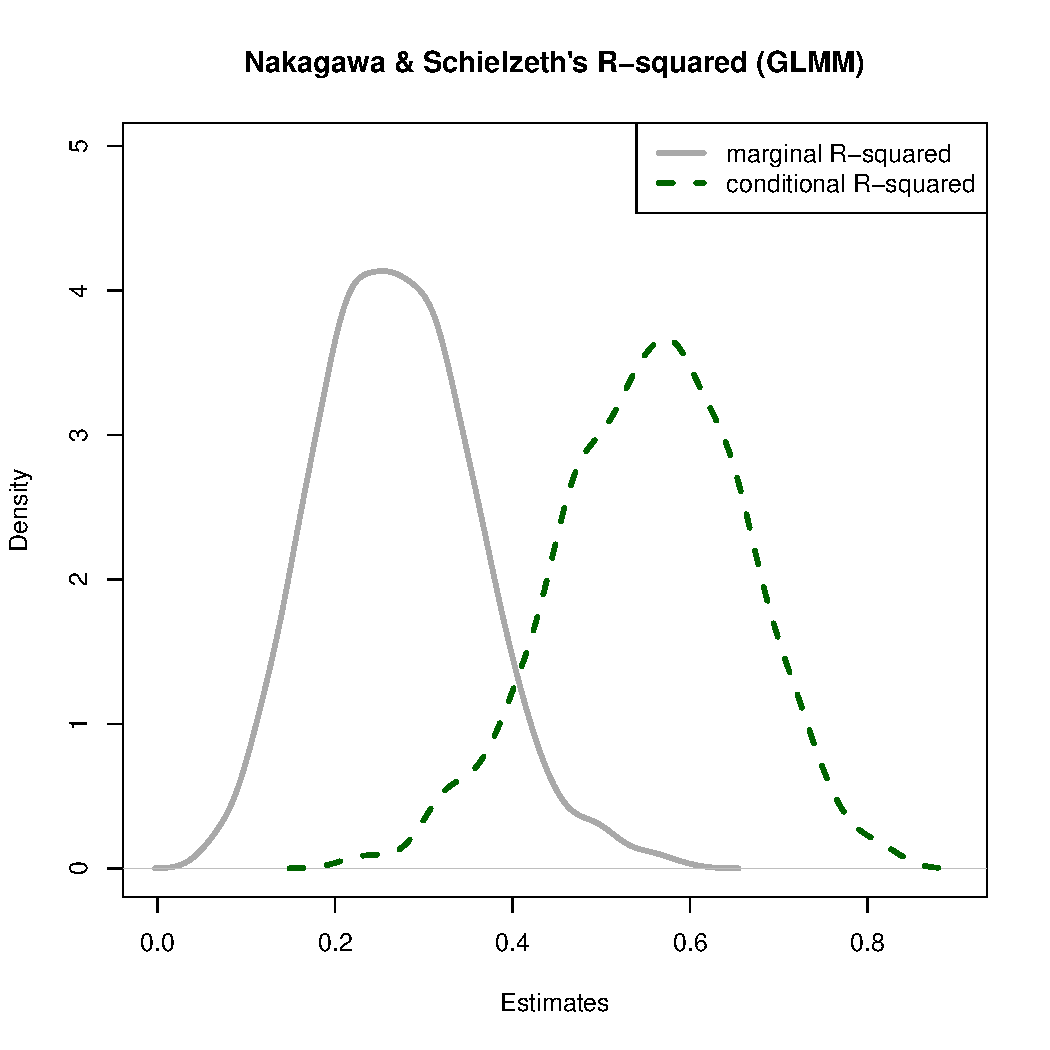
\includegraphics[width=0.6\textwidth]{graphics/rsqglmmj5i20}
  \caption{Distribution of Nakagawa \& Schielzeth's $R^2$ in the simulations described in Section~\ref{sec:choosingbetweenrandomandfixedeffects}}
  \label{fig:rsqglmmj5i20}
\end{figure}

\begin{figure}[!htpb]
  \centering
  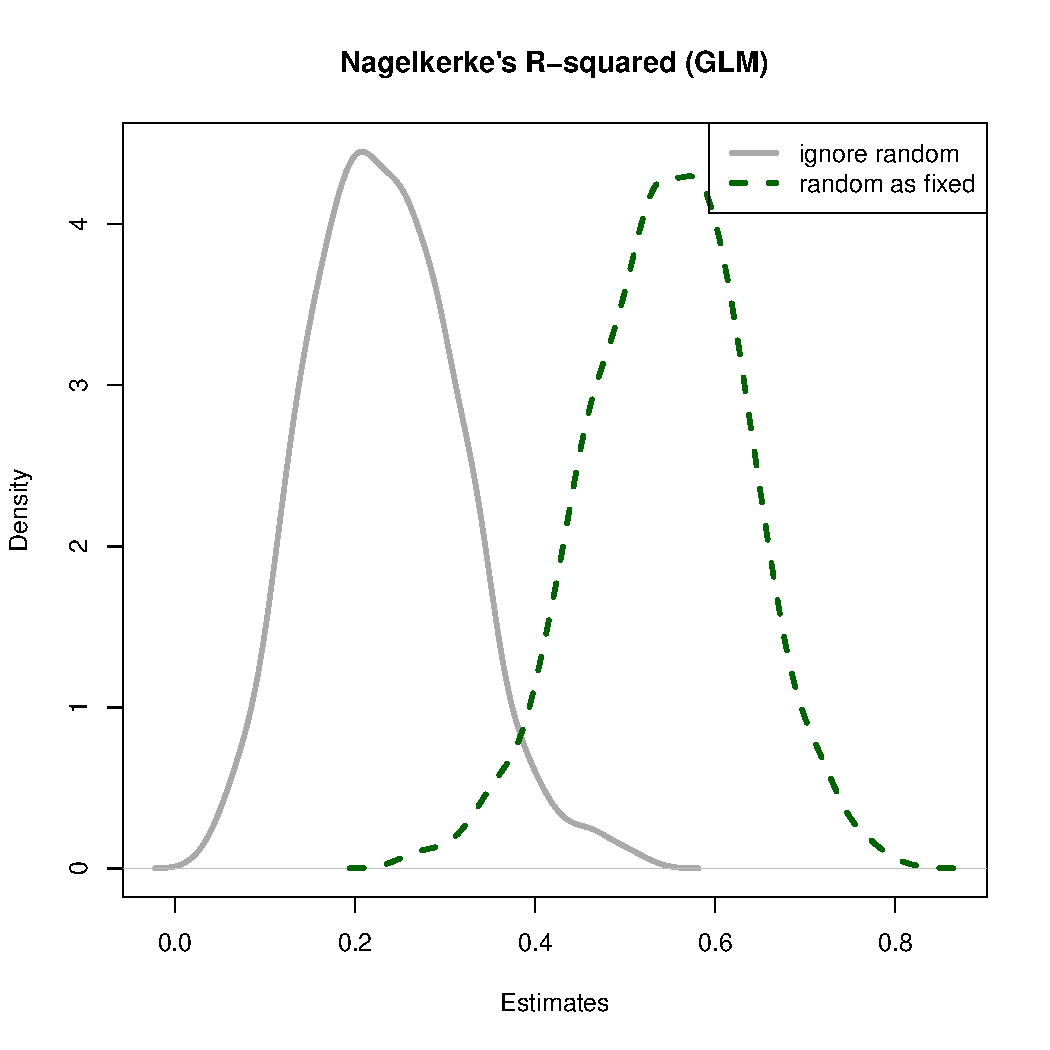
\includegraphics[width=0.6\textwidth]{graphics/rsqglmj5i20}
  \caption{Nagelkerke's $R^2$ in the simulations described in Section~\ref{sec:choosingbetweenrandomandfixedeffects} for a GLM that ignores the grouping factor and a model that includes it as a fixed effect}
  \label{fig:rsqglmj5i20}
\end{figure}

\subsubsection{More complex models}
\label{sec:morecomplexmodels}


\paragraph{Varying intercepts and slopes}

While it is possible to have just a varying slope, this is rarely useful, and we discuss only varying-intercept and varying-slope (VIVS) models.
An example of when a VIVS model might be useful was given in Section~\ref{sec:randominterceptsandslopes}, and readers might want to review this before continuing on.
We extend the simple model from (\ref{eq:glmm01}), and the fixed effect coefficients for which a random slope is specified simply receive group indices; see (\ref{eq:glmm05}).
Instead of estimating a fixed coefficient, coefficients are predicted and assumed to come from a random (normal) distribution.
We use $\beta_{d:l}$ to denote the coefficient for givenness varying by lemma.

\begin{equation}
  P(y^i=1)=logit^{-1}(\alpha_{l}^{j[i]}+\beta_{d:l}^{j[i]}\cdot x_d^i)
  \label{eq:glmm05}
\end{equation}

A source of problems in VIVS models is the fact that in addition to the variance in the intercepts and slopes, the covariance between them has to be estimated.
If in groups with a higher-than-average intercept, the slope is also higher than average, they are positively correlated, and vice versa.
These relations are captured in the covariance.
Condition (\ref{eq:glmm06}) is added, where the indices $l$ and $d:l$ are omitted for readability.

\begin{equation} 
  \left( \begin{smallmatrix} \alpha^j \\ \beta^j \end{smallmatrix}\right) \sim
    \left(
    \left( \begin{smallmatrix} \mu_{\alpha}\vphantom{\beta^j} \\ \mu_{\beta}\vphantom{\beta^j} \end{smallmatrix} \right), 
      \left( \begin{smallmatrix} \sigma_{\alpha}^2 & \rho\sigma_{\alpha}\sigma_{\beta} \\
	\rho\sigma_{\alpha}\sigma_{\beta} & \sigma_{\beta}^2 \end{smallmatrix} \right)
    \right)
  \label{eq:glmm06}
\end{equation}

(\ref{eq:glmm06}) says that the joint distribution of the intercepts $\alpha^j$ and the slopes $\beta^j$ follows a bivariate normal distribution with means $\mu_{\alpha}$ and $\mu_{\beta}$.
The variance in the intercepts is $\sigma_{\alpha}$, the variance in the slopes is $\sigma_{\beta}$, and the coefficient for the covariance between them is $\rho$.
Figure~\ref{fig:multnorm} shows the bivariate density distributions for two (1) negatively correlated, (2) non-correlated, and (3) positively correlated normally distributed variables.

\begin{figure}[!htpb]
  \centering
  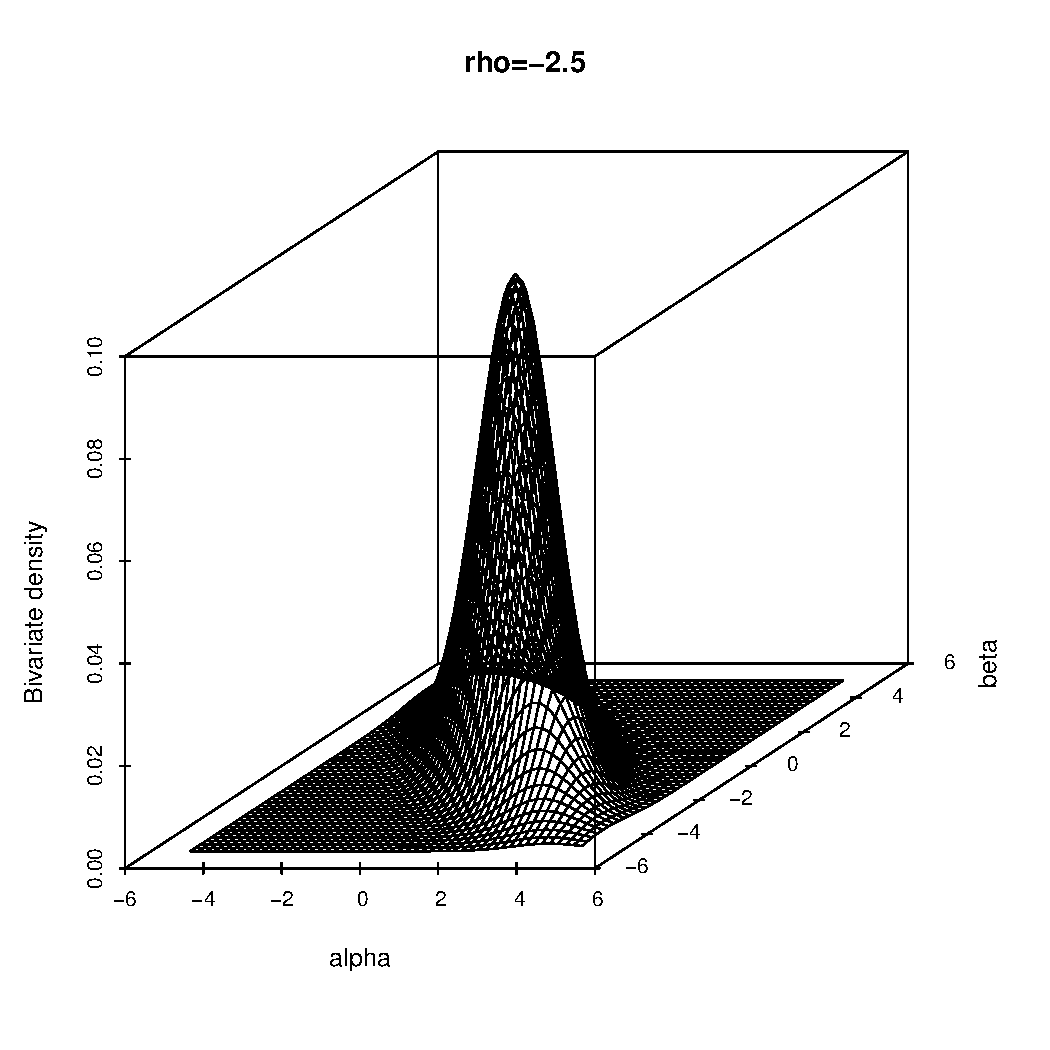
\includegraphics[width=0.33\textwidth]{graphics/multnorm1}~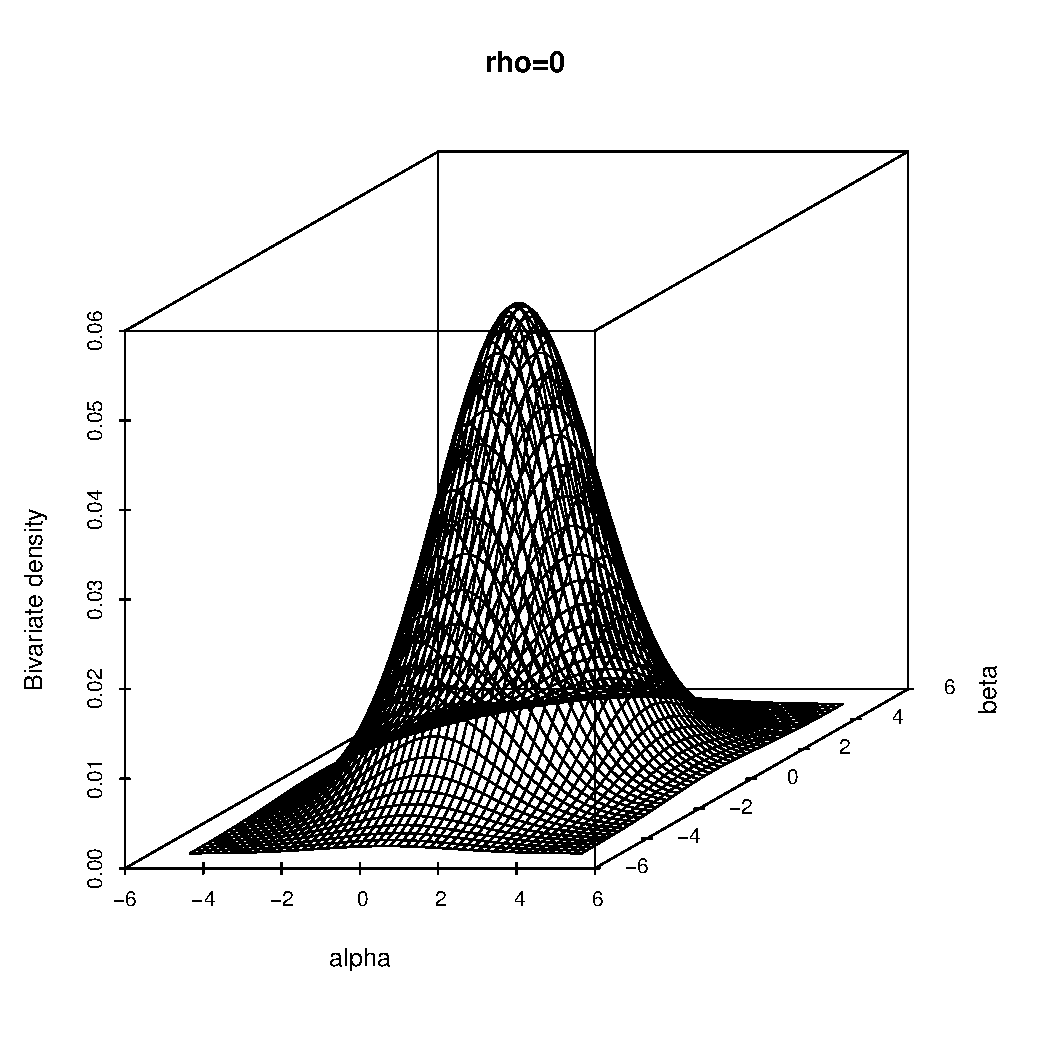
\includegraphics[width=0.33\textwidth]{graphics/multnorm2}~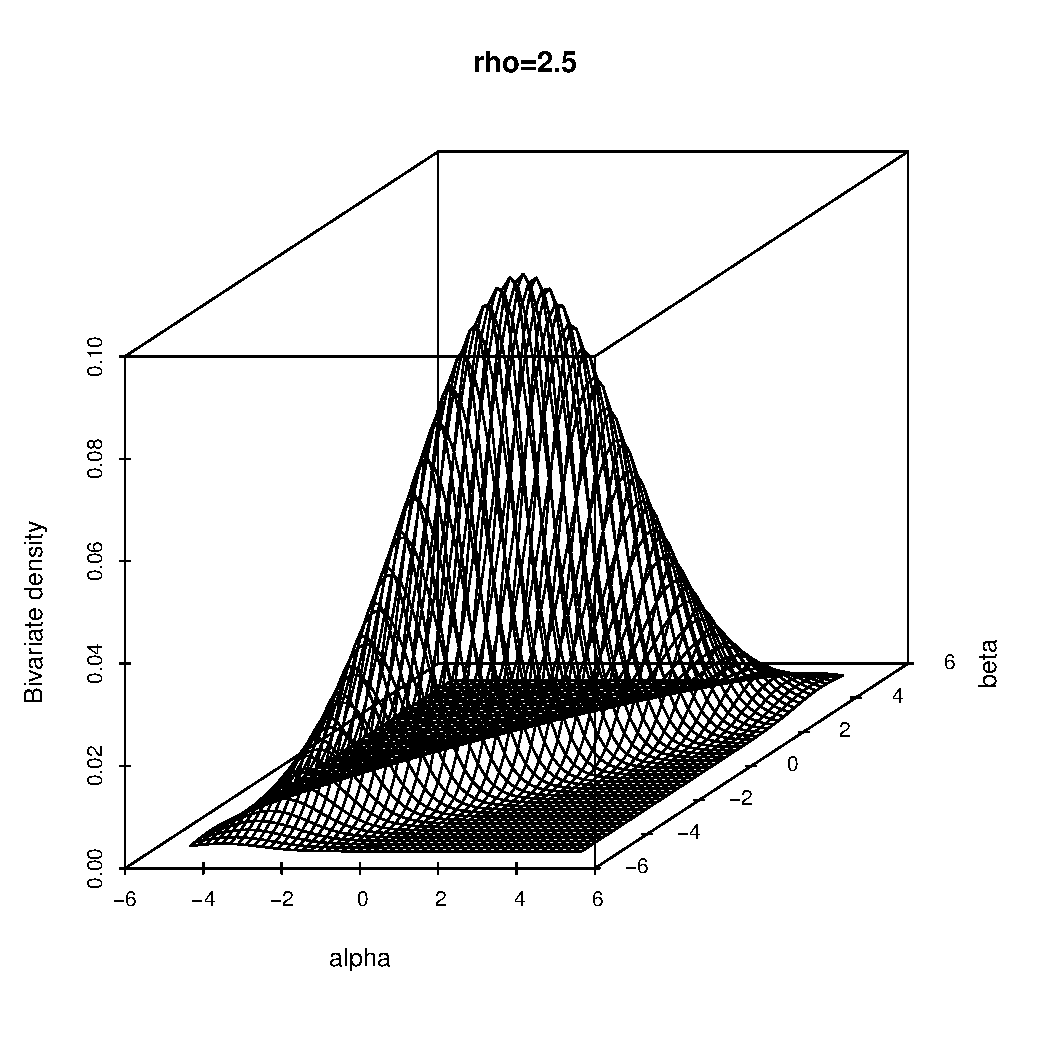
\includegraphics[width=0.33\textwidth]{graphics/multnorm3}
  \caption{Bivariate normal density distribution with different correlation coefficients $\rho$; $\sigma_{\alpha}=\sigma_{\beta}=3$; $\mu_{\alpha}=\mu_{\beta}=0$}
  \label{fig:multnorm}
\end{figure}

The number of variance parameters to be estimated thus obviously increases with more complex model specifications, and the estimation of the parameters in the presence of complex variance-covariance matrices requires considerably more data than estimating a single variance parameter.
The estimator might converge, but typically covariance estimates of $-1$ or $1$ indicate that the data was too sparse for a successful estimation of the parameter.
In this case, the model is \textit{over-parametrised} and needs to be simplified.

\paragraph{Nested and crossed random effects}

As it was explained in Section~\ref{sec:crossedandnestedeffects}, nested random effects are adequate when grouping factors are nested within other grouping factors.
Technically, while varying slopes can be understood as interactions between a fixed and a random effect, nested random intercepts can be understood as interactions between two or more random effects.
Crossed random effects are just several unrelated random effects.
(\ref{eq:glmm07}) shows the model specification, extending (\ref{eq:glmm01}) with a varying intercept $\alpha_s$.
This could be for example semantic classes which nest individual lemmas.
It could also be another grouping factor for speaker, completely unrelated to the lemmas.

\begin{equation}
  P(y^i=1)=logit^{-1}(\alpha_{s}^{k[i]}+\alpha_{l}^{j[i]}+\beta_d\cdot x_d^i)
  \label{eq:glmm07}
\end{equation}

The difference is that in the nested case, $k[i]=k[j]$, \ie the level of the nesting factor can be selected based on the nested factor as well as based on the single observation.
As was mentioned in Section~\ref{sec:crossedandnestedeffects}, the question is rather one of how the way the data are organised.

\paragraph{Second-level predictors}

In Section~\ref{sec:hierarchicalormultilevelmodels}, situations were introduced where the random effects themselves can be partially predicted from fixed-effects.
In this case, an additional linear model is specified for the random effect instead of the simple normal distribution predictor.
We extend (\ref{eq:glmm01}) by a predictor $\gamma_f$ for the lemma frequency.
The lemma frequencies themselves we denote by $u_f$, and we index them with $j$, just like the verb lemmas.
This is reasonable because for each verb lemma, there is exactly one frequency.
The first-level model specification remains the same, namely (\ref{eq:glmm08}).

\begin{equation}
  P(y^i=1)=logit^{-1}(\alpha_{l}^{j[i]}+\beta_d\cdot x_d^i)
  \label{eq:glmm08}
\end{equation}

However, instead of (\ref{eq:glmm02}), the varying intercept is predicted from (\ref{eq:glmm09}).

\begin{equation}
  \alpha_l^j\sim N(\gamma_0+\gamma_f\cdot u_f^j,\sigma_l^2)
  \label{eq:glmm09}
\end{equation}

Instead of just the mean of the $\alpha_j$ values, the model in (\ref{eq:glmm09}) specifies a second-level intercept $\gamma_0$ and a second-level fixed coefficient $\gamma_f$.

